\documentclass[conference]{IEEEtran}
\IEEEoverridecommandlockouts
% The preceding line is only needed to identify funding in the first footnote. If that is unneeded, please comment it out.
\usepackage{cite}
\usepackage{amsmath,amssymb,amsfonts}
\usepackage{algorithmic}
\usepackage{graphicx}
\usepackage{textcomp}
\usepackage{xcolor}
\usepackage{float}
\usepackage{subfig}

\pagestyle{plain}


\def\BibTeX{{\rm B\kern-.05em{\sc i\kern-.025em b}\kern-.08em
    T\kern-.1667em\lower.7ex\hbox{E}\kern-.125emX}}
\begin{document}

\title{Identifying Hate Speech Categories On Social Media\\
}

\author{\IEEEauthorblockN{Jack Ryan Cracknell}
\IEEEauthorblockA{\textit{School of Electronic Engineering and Computer Science} \\
\textit{Queen Mary University of London}\\
London \\
jcracknell123@gmail.com / EC20046@qmul.ac.uk}
}

\maketitle

\begin{abstract}
With the ever increasing popularity of social media within our society, online user-to-user interaction has never been so prevalent. Whilst social media sites possess many positives; under the surface exists a growing population of people using such platforms to cause harm. Through natural language processing models, it is possible to detect when a social media post contains hate speech. These models can be used to autonomously moderate sites and remove hateful or offensive messages, lowering the burden on human moderation. In this paper, machine learning models will be trained and compared in the task of identifying the specific type of hate speech that a message contains. Through this model, social media sites can alter their methods of stemming hate speech on their sites by strongly targeting the most rampant types of hate speech. \\
\end{abstract}

\begin{IEEEkeywords}
Hate speech; social media; multi-class classification; text preprocessing 
\end{IEEEkeywords}

\section{Introduction}
Hate speech has been defined as 'any communication that disparages a person or a group on the basis of some characteristics such as race, colour, ethnicity, gender, sexual orientation, nationality, religion, or other characteristics' \cite{9}. \\
With the ever growing population of social media sites, there has been an explosion of posts that have been uploaded to them. Due to this, there has also been an increase in the amount of hateful activity online. Some of this hateful activity has been broadcast in real time on social media sites, such as the Christchurch shooting in 2019 \cite{12}. In response to this, the government of the United Kingdom has utilised anti-hate speech laws which forbids both the expression of hatred towards someone based on given characteristics\cite{11} and also any threatening communication\cite{5}. These laws have been used to arrest and prosecute those who write hateful messages online\cite{14}. Successfully identifying these hate speech messages through machine learning models aids in removing not only the messages themselves but also similar posts and sentiments, stemming the amount of hate that can be spread. Having a state-of-the-art hate speech classification model may also increase the speed and accuracy at which social media sites can identify possible perpetrators of hateful actions in the real world. These metrics are key in reducing potential real world offences, since many individuals who commit violent hate crimes have previously posted hate speech online\cite{8}. Furthermore, having the ability to classify hate speech posts to their most relevant subclass may give insight into how social media sites can alter their moderation systems in order to lower a certain type of hate speech.\\
Before automatic natural language processing (NLP) models were introduced, websites would aim to block hate speech by having filters around specific words and phrases, though this is method extremely time consuming and also scales poorly due to the quick evolution of language \cite{13, 2}. Therefore an effective NLP model must be adaptable to new language and efficient in parsing through huge datasets. \\
In this paper, a systematic approach is taken to collecting multiple performance metrics for various machine learning algorithms on a dataset of tweets. The dataset used is a merge between Waseem and Hovy\cite{16} and Atai and Jefroykin\cite{1}. The merge was done to create a dataset that has four total classes; \textit{Sexism}, \textit{Racism}, \textit{Homophobia} and \textit{Neither}.
This work will compose what can be used as baseline statistics for a standard hate speech detection task through comparison of both traditional and \textit{state-of-the-art} techniques. An overall conclusion will be judged on the results collected, in addition to areas further work could focus upon. 


\section{Background and related work}
There are various NLP methods for tackling hate speech online. Some classical approaches include Logistic regression, Support Vector Machines and Bayes models. In recent years, neural network models have become the industry standard state-of-the-art approach \cite{19}, although in some cases, the results given by neural networks can be difficult to interpret \cite{10}. This paper will examine comparisons between both of these approaches.

\subsection{Related work}
This section is tasked with bridging the gap between the research done in this paper, and other work that is currently out there.\\

The first key piece of related work is the paper is \textit{Hateful symbols or hateful people?} authored by Zeerak Waseem and Dirk Hovy in 2016. This paper introduces one of the datasets used in this project - tweets attributed to the classes; racism, sexism and neither. In addition to this, they set out some fundamental rules of what can be considered offensive text. Through the use of a logistic regression classifier and multiple features such as n-grams, gender and geographic distribution, they achieved f1 results ranging from mid 64-74\%\cite{16}.
A paper by Gilbert et al. in 2018 investigated the type of hate speech used on a well known white supremacy internet forum. Gilbert et al. supply a hand-annotated dataset with their work. Their paper compares SVM, Convolutional Neural Networks (CNN) and a type of Recurrent Neural Network known as LSTM or Long Short-Term Memory \cite{7}. LSTM models were previously state-of-the-art for natural language processing, though now transformer based models such as BERT have become the model of choice \cite{17}.
Finally, this paper by Basile et al, 2019 describes their work on the annual SemEval competition, specifically task 5 - detection of hate speech against women and immigrants\cite{3}. Their paper looks into both English and Spanish twitter data, and attempts to classify hate speech as well as semantically evaluating aggressive tweets.

\subsection{Classification models}
\paragraph{\textbf{Logistic Regression}} This classifier is a supervised machine learning algorithm which predicts a target probability value between 0 and 1. This is achieved through the following equation.
\[y = \frac{\exp(\beta_{0} + \beta_{1} \text{data})}{1 + \exp(\beta_{0} + \beta_{1} \text{data})}\]
The data that will be used in this project will be preprocessed tweets, $\beta_{0}$ is the bias term and $\beta_{1}$ is the coefficient term for the input data. This coefficient term is learned from the training data.

For a binary classification task, \textit{y} will be the probability of the default class. The default class will be the tweet containing no hate speech. This is represented by the equation \[ P(Hate=False | Tweet) \]
\noindent
Where P $<$ 0.5, the sample will be classified as 0 - no hate\\
Where P $>=$ 0.5, the sample will be classified as 1 - hate\\

\noindent
\\The methodology differs slightly when more than two classes are involved as logistic regression does not natively support multi-class classification. This new technique is named \textit{'one vs rest'} - hereby referred to as OvR splits the problem up into multiple binary classification tasks.\\
\begin{itemize}
  \item Binary Problem 1: Class1 vs [Class2, Class3, Class4]
  \item Binary Problem 2: Class2 vs [Class1, Class3, Class4]
  \item Binary Problem 3: Class3 vs [Class1, Class2, Class4]
  \item Binary Problem 4: Class4 vs [Class1, Class2, Class3]\\
\end{itemize}

OvR takes a single classifier per class, where samples classified as the current target class are represented as positive, and all other samples are negative\cite{4}. Each classifier produces a confidence score. The predicted class label is chosen by the corresponding highest confidence model. OvR has some scalability issues that become apparent with very large class sets or slow models due to the need of creating a single model for each label, though these issues do not appear in this project.\\

\paragraph{\textbf{Support Vector Machine}} SVMs are a type of supervised learning algorithm that aims to predict a target class by separating data samples by a hyperplane. SVMs decide on the most optimal hyperplane by selecting that which has the largest distance from data samples on each side of the separator. \textit{'Support vectors'} refer to samples which are closest to the separating line. The position of these vectors changes the size of the margin depending on their location. These can be seen in figure \ref{fig:support_vectors},

\begin{figure}[h]
    \centering
    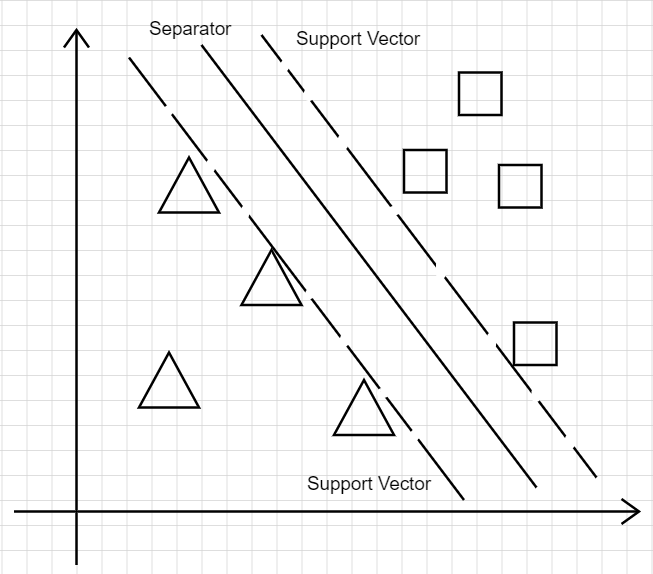
\includegraphics[width=0.35\textwidth]{Support_vectors.png}
    \caption{Example of a linear separator with support vectors}
    \label{fig:support_vectors}
\end{figure}

When more than two classes are introduced to an SVM, the classifier takes the same approach as logistic regression, utilising OvR. In this case, a separating margin will be drawn between the target class sample and the \textit{rest} of the dataset. The label with the corresponding highest confidence margin will be chosen as the prediction.\\

\paragraph{\textbf{Naive Bayes}}
Naive Bayes (namely GaussianNB which will be used in this project) is a supervised learning algorithm based on the \textit{Bayes' Theorem}

\[P(A|B) = \frac{P(A) \cdot P(B|A)}{P(B)}\]

In the above equation, P(A) is the probability of A occurring, P(B) is the probability of B occurring, P(A$|$B) is the probability of A given B has occurred and P(B$|$A) is the probability of B given A has occurred. This equation can also be written in context of this project.

\[P(Hate|Tweet) = \frac{P(Hate) \cdot P(Tweet|Hate)}{P(Tweet)}\]

Tweet contains a feature vector containing the preprocessed words in each tweet sample. In Naive Bayes, there is an assumption of independence between the data samples supplied, specifically, each word in the tweet would contribute independently to the class prediction. Using this independence assumption, we calculate the likelihood of a class label being predicted by the sum of the probabilities of observing each word in the tweet

\[P(Hate|word_1 ... word_n) = \] 
\[P(Hate) \cdot P(word_1|Hate)... P(word_n|Hate)\]

Bayes' models will calculate probabilities for all classes through these equations, making it well suited for both binary and multi-class problems.
The Bayes' classifier that has been used in this project is Gaussian Bayes' which adds the assumption that the continuous values associated with each class are in the form of a Gaussian distribution. The application of this is particularly interesting when the tweet text is vectorised.\\

\paragraph{\textbf{Transformer model}}
The current \textit{state-of-the-art} models in natural language processing are transformers. Transformers use \textit{attention}, which is a method of giving more weight to what are deemed to be more important parts of the data, while less important parts are neglected. Transformer models tend to be designed for tasks that have sequential data, which further cements their application to natural language processing tasks. Attention layers use context for a given position in the input data. Through the architecture, the layer can use preceding states and weights to give relevancy about data that is not directly adjacent. Transformers also scale well by implementing paralellisation, making them particularly time efficient in comparison to other neural network models \cite{15}.
Transformers use the encoder-decoder architecture.

\subsubsection{\textbf{Encoder}} It is the encoders job to iterate through the input one layer at a time, creating encodings which link relevant pieces of data together. The first layer uses the data embedding while each subsequent layer uses the output of the previous encoder.

\subsubsection{\textbf{Decoder}} The decoder takes the encodings and creates an output using the newly formulated information. These layers contain the attention functions which aim to retrieve the additional information created by the encoder.\\

This project uses a specific type of transformer model known as BERT (Bidirectional Encoder Representations from Transformers), created by Google in 2018\cite{6}. BERT has two models which have been pre-trained on data from BooksCorpus\cite{18} as well as the English wikipedia site. 

\begin{itemize}
  \item \textit{Base} contains 12 encoders with 12 bidirectional attention heads
  \item \textit{Large} contains 24 encoders with 16 bidirectional attention heads.\\
\end{itemize}

BERT differs slightly from the traditional transformer model as it does not include a decoder in the architecture. A decoder is not needed as BERT is used to generate a language model. A task specific decoder must be formulated whenever applying BERT to a piece of work. A visual representation of how BERT is applied to a tweet from the dataset in project is shown in figure 2.

\begin{figure}[h]
    \centering
    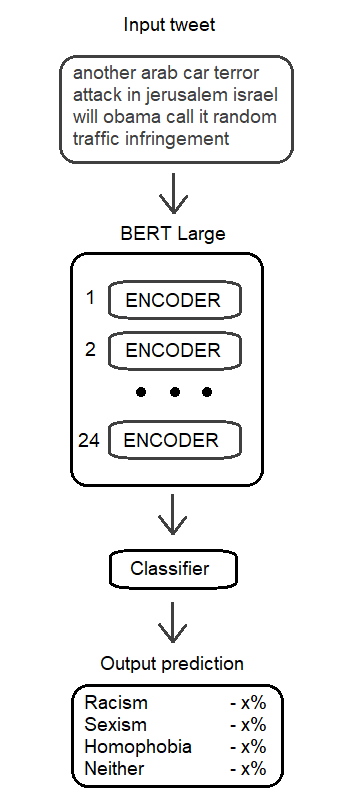
\includegraphics[width=0.35\textwidth]{BERT_model.png}
    \caption{BERT model architecture}
    \label{fig:bert_architecture}
\end{figure}


\subsection{Word embedding}
Word embeddings are a way to represent words in a text as a number or vector rather than their initial string format. The main idea which underpins word embeddings is that words that have similar meaning will be closer together in vector space. Many different vectorisers exist, though three have been chosen for this project.\\

\paragraph{\textbf{Count vectorisation}} This technique is simply word representation, a vector is built with size equal to the amount of unique words in the text. When a word appears in the corpus, it will be added to the vector representation matrix, if this word appears again, the count will be increased. Using this method on a large text corpus tends to make each count vector very sparse. Count vectors contain no information about the relation or similarity between words, the only information stored is whether the word appears or not. An example of a count vector is shown below.

\[Vocabulary = \{thanks; hello; for; reading; thanks\} \] 
Vector representation matrix:
\begin{table}[H]
\centering
\begin{tabular}{|l|l|l|l|}
\hline
thanks & hello & for & reading \\ \hline
2      &   0   &  0  &    0 \\ \hline
0      &   1   &  0  &    0 \\ \hline
0      &   0   &  1  &    0 \\ \hline
0      &   0   &  0  &    1 \\ \hline
\end{tabular}
\end{table}

If we then have a sentence in our dataset which consists of the text "reading for homework", the feature vector would have a size of 4 - the length of the vocabulary and have a 1 indices 2 and 3.
\[ [0, 0, 1, 1]\]

Given a much larger corpus vocabulary, it is evident that the count vector can see increasing amounts of sparsity. This is quite prevalent in the context of this project as the vocabulary of all words in the dataset is quite large in comparison with the average amount of words in a tweet.\\

\paragraph{\textbf{TFIDF}}
TFIDF is the acronym for Term Frequency Inverse Document Frequency. This is combination of two other statistical metrics.\\
\textbf{Term Frequency} - a count of how many instances of a word appear in total within a text. This is formally represented as:

\[ TF = \frac{Number\: of\: times\: a\: word\: appears\: in\: text}{total\: number\: of\: words\: in\: text}\]

\textbf{Inverse Document Frequency} - IDF is a metric that is concerned with weighting how much information a word in a text can give. Since IDF is an inverse fraction, it supplies a higher weighting for rarer terms whilst giving a lower weight to more frequent terms. Formally:

\[ IDF = log \frac{total \: number \: of \: texts \: in \: a \: corpus}{number \:
of \: texts \: where \: word \: appears}\]

Finally, these two terms are combined to calculate TFIDF:

\[ TFIDF = TF \cdot IDF \]

A higher TFIDF will mean that the word is more relevant in relation to the text\\

\paragraph{\textbf{Word2vec}}
Word2vec is a dual layer neural network which processes text into numerical feature vectors\textbf{CITE HERE}. One key idea behind word2vec is that once vectorised, similar words will be distributed near each other in vector space. The similarity can be measured by calculating the cosine similarity.

\[ Cos\theta = \frac{A \cdot B}{|| A || \: || B ||}\]

Word2vec can be be pre-trained on a large text corpus and then utilised on a dataset through transfer learning, or can be trained on the domain-specific data in the task at hand. Given the small size of the dataset in this project, a pre-trained word2vec embedding has been used through the spaCy python library. \\

\section{Methodology}
The main focus of this paper is to experiment and discuss the effectiveness of various machine learning models on the task of identifying hate speech categories in a dataset of tweets. Given this is quite a large and open-ended task, the research has been split up into two parts - a binary classification task and a multi-class classification task.

The reasoning behind this is that the binary classification task will act as a benchmark. Metrics taken from the initial research can be used as comparison when evaluating and concluding the results. How well a classifier is able to distinguish between hate and non-hate should be a good indicator of what the upper limit of the performance metric we should see in a multi-class environment. This is due to the added complexity when increasing the number of class labels, if a model struggles to distinguish between hate and non-hate, it is unlikely that the same model will be able to accurately identify the type of hate speech contained in text.

Furthermore, machine learning algorithms are not the only natural language processing techniques that will be used. Different methods of word vectorisation will be experimented to see their effect on a small, niche dataset in comparison to previous research on large common-task datasets as mentioned in the background section. 

\subsection{Dataset}
The two datasets that were merged to create the data for this project were chosen because of their good application to the tasks they were created for as well as having a wide variety of various types of hate speech. By merging two sources, a unique dataset has been made. One that contains tweets from three of the biggest hate speech types. This collection of tweets could be further extended for other tasks if necessary but has the luxury of being directly applicable. In addition to this, the tweets contained in the dataset have been stored physically so that there is still a record tweets that get removed from the site. \\

A small exploratory analysis has been completed into the dataset that is used in this project. The aim of this task was to gain additional insight into the contents of the dataset as well as it's distribution. Below shows an example of the dataset after the data preprocessing task which is outlined within this section.

\begin{table}[H]
\centering
\begin{tabular}{|l|l|l|l|l|l|}
\hline
{} & id & text & Annotation & clean\_text & Hate \\ \hline

0 & 5969... &  I just found... & Neither & i just found t... &  0 \\ \hline
1 & 5758... &  @wetsprocket... & Neither & every time th... & 0 \\ \hline
2 & 5952... &  ok time to w... & Neither & ok time to wr... & 0 \\ \hline
\end{tabular}
\caption{\label{tab:dataset-head}Samples from core dataset columns.}
\end{table}

In this table, \textit{id} relates to the tweet id attached to the tweet. This ID can be used to search for the tweet through the twitter API. \textit{Text} is the original tweet string before any preprocessing. \textit{Annotation} is the type of hate speech the tweet falls under. This can be either; sexism, racism, homophobia or neither. \textit{Clean\_text} is the preprocessed version of \textit{text}. Finally, \textit{hate} is a binary column, showing 0 if the tweet contains no hate, and 1 if the tweet contains hate.

\begin{table}[H]
\centering
\begin{tabular}{|l|l|l|}
\hline
{} & clean\_text\_sl & postags \\ \hline

0 & found perfect renta... & found\_VBN perfect\_JJ rental\_JJ... \\ \hline
1 & every time dis ... &  every\_DT time\_NN discover\_RP...
 \\ \hline
2 & ok time write code bb... & ok\_JJ time\_NN write\_JJ code\_NN ...
 \\ \hline

\end{tabular}
\caption{\label{tab:extra-cols}Extended columns used for specific classifiers.}
\end{table}

Some extra columns were created to be used for various classifiers. \textit{clean\_text\_sl} contains the text from \textit{clean\_text} but with the added preprocessing of the removal of stopwords as well as lemmatisation. This column is used for the vectorisation and input of traditional machine learning models in this project, while \textit{clean\_text} is used for BERT. \\
\textit{Postags} contains the text from \textit{clean\_text\_sl} but each word has the Part-Of-Speech tag connected to it. This column is used in the binary classification task. A PoS tag is a way of encoding grammatical rules to the text they are associated to. In theory, having a PoS tag associated with a word can provide extra information to the classifier, but in reality, this is not always the case.

The below table shows the distribution of how many tweets are in each class.

\begin{table}[H]
\parbox{.45\linewidth}{
\centering
\begin{tabular}{|l|l|}
\hline
{} Annotation & Count  \\ \hline
Neither    &        5740 \\ \hline
Sexism     &         911 \\ \hline
Racism     &          98 \\ \hline
Homophobia &          87 \\ \hline
\end{tabular}
\caption{\label{tab:multi-class-distribution}Multi-class \\distribution.}
}
\parbox{.45\linewidth}{
\centering
\begin{tabular}{|l|l|}
\hline
{} Annotation & Count  \\ \hline
0    &     5740 \\ \hline
1    &     1096 \\ \hline
\end{tabular}
\caption{\label{tab:binary-class-distribution}Binary class distribution.}
}
\end{table}

A large class imbalance was purposefully chosen as this is realistic to how a real-world hate speech detection task would have to operate. This class imbalance is a hurdle that exists and will be explored in classification.\\

Table V shows the average tweet character lengths contained in each subclass of hate. 

\begin{table}[H]
\centering
\begin{tabular}{|l|l|}
\hline
 Annotation &  Average Tweet Length \\ \hline
 Homophobia &             149  \\ \hline
    Neither &             91  \\ \hline
     Racism &             106  \\ \hline
     Sexism &             97  \\ \hline
\end{tabular}
\caption{\label{tab:tweet-length}Average tweet length across classes.}
\end{table}

While it can be seen that sexism and racism have a much lower average character length, their frequent words appear much more. A further look into the dataset shows that many of the homophobic tweets contained links to YouTube videos or other websites, which has bumped up their average length considerably. The fact that many homophobic tweets contained links may be something to consider when assessing how well a classifier was able to perform. 

\begin{table}[H]
\parbox{.32\linewidth}{
\centering
\begin{tabular}{|l|l|}
\hline
{} Word & Count  \\ \hline
feminazi    &   570 \\ \hline
rt          &   150 \\ \hline
mkr         &   126 \\ \hline
woman       &   83 \\ \hline
\end{tabular}
\caption{\label{tab:sexism-hate-words}\\Common \\sexist words.}
}
\parbox{.32\linewidth}{
\centering
\begin{tabular}{|l|l|}
\hline
{} Word & Count  \\ \hline
coon   &    69 \\ \hline
arab   &    17 \\ \hline
rt     &    16 \\ \hline
terror &    13 \\ \hline
\end{tabular}
\caption{\label{tab:racism-hate-words}\\Common \\racist words.}
}
\parbox{.32\linewidth}{
\centering
\begin{tabular}{|l|l|}
\hline
{} Word & Count  \\ \hline
gay        &  40 \\ \hline
homophobe  &  15 \\ \hline
marriage   &  11 \\ \hline
day        &  10 \\ \hline
\end{tabular}
\caption{\label{tab:homophobic-hate-words}\\Common \\homophobic words.}
}
\end{table}

Looking at the most common words for each subclass, it can be noticed that the most frequently appearing words seem to show up three to four times more than that of the second place word. These \textit{trigger words} are likely one of the lookup phrases used by the initial dataset creators and are invaluable to machine learning classifiers when trying to detect patterns.

\subsection{Data preprocessing}
Data preprocessing is a key part of any natural language processing task. IBM programmer George Fuechsel coined the phrase "garbage in, garbage out" - referring to how the quality of the input data is directly related to the quality of the output result. This is particularly apparent in the field of NLP.\\
When text data is analysed, only certain parts of the text can give clues as to what words mean. Therefore preprocessing the data as to reduce the amount of low quality words, phrases or other strings is crucial.\\
Multiple preprocessing methods have been used in this task, these methods are outlined as follows:

\begin{itemize}
  \item \textbf{Hyperlink removal} - Many tweets in this dataset contain links to other websites. In addition to this, twitter host images that are uploaded directly to the tweet, when the text is taken from a tweet, this picture is put into a link which redirects to the image. While images may be relevant to the tweet content, they are not useful when analysing words. Any word that begins with http or https has been removed from the tweet text. The rest of the tweet remains.
  
  \item \textbf{Tag removal} - Twitter has functionality to tag other users in tweets. Once sent, this tweet will notify the user that has been tagged. This information provides no contextual information about what is being said and so has been removed.
  
  \item \textbf{Punctuation removal} - Since only the words in the tweet are being analysed, it makes sense to remove any punctuation as this could add noise. Specifically when some vectorisation methods will take "word" and "word." to be different items. All punctuation has been removed - no symbols exist in the cleaned tweets.
  
  \item \textbf{Numerical value removal} - As with punctuation, numbers in tweets can just add noise to the dataset. In addition, some issues may occur when trying to vectorise a numerical feature.
  
  \item \textbf{Empty tweet removal} - Any rows in the dataset that have NaN or empty values have been removed as any imputation methods would not be accurate for this type of task. Empty cells may exist in the initial data or could have been created by the data preprocessing described above. 
  
  \item \textbf{Lowercase tweets} - Further tweet normalisation has been done by removing any capitalisation in the dataset. This is to make sure there is no discrepancy between "WoRd" and "word".
  
  \item \textbf{Stopword Removal} Stopwords are common words in a domain language that appear much more frequently than other words. Examples of these in the English language include "and", "the" or "it". These words do not provide much use to machine learning models at the single word level. The dataset splits here, in addition to the previous preprocessing methods, stopword removal and the following lemmatisation are added to a new column.
 
  \item \textbf{Lemmatisation} - Lemmatising words refers to the grouping together of the inflected forms of words. This can be useful in NLP tasks as it reduces the amount of items in vector space. An example of lemmatising words would be "found" and "finding" would both become "find". 
  \\ \\
  The reason for stopword removal and lemmatisation being in an additional tweet column is that while it is useful for models that use word vectorisation, the BERT model that is experimented with on the multi-class classification analyses context between words in a tweet. Therefore it is important to keep as many original words as possible.
  
  \item \textbf{Binary hate column} - Finally, given that a small binary classification task is included in this project, an additional label column has been added to facilitate this. The original dataset has "Annotation" as the labels, which is multi-class. To solve this, any label in this column which is "Neither" will be given a 0 while others are given a 1.
\end{itemize}


\subsection{Grid search parameter optimisation}\label{AA}
In this project, three machine learning models that have a large number of potential hyperparameters have been used. These are the previously mentioned \textbf{SVM}, \textbf{Logistic Regression} and \textbf{Naive Bayes}. Instead of manually testing these hyperparameters to find the optimal settings, a grid search technique can be used to increase the time efficiency of this project.  Grid search is an exhaustive search over all specified parameter combinations. The data is collected as to which parameter combination is the best for a given metric. These parameters can then be used in the future.

\section{Experiments and Results}

\subsection{Binary Classification}
The first experiment was a binary classification task. The purpose of this was to explore how the data would respond to classical machine learning techniques as well as gauge what the baseline precision, recall and macro\_f1 metrics would be. While we have a different amount of classes for the multi-class experiment, the results should be strongly correlated since if a classifier is unable to correctly classify a tweet as hate speech, it will be unlikely that the same classifier will identify the specific type of hate.

Throughout the whole of this project, the two main metrics that will be compared are recall and macro f1 score. Precision will also be analysed, but to a lesser extent. That is because this paper puts more emphasis on correctly identifying hate speech messages over non-hate.  Different parameters have been experimented with as part of this task, in addition to the utilisation of Part-of-Speech tagging.\\

Table IX shows the results collected for each model run with count vectorisation word embeddings used as inputs.

\begin{table}[H]
\centering
\begin{tabular}{|l|l|l|l|}
\hline
model              & precision & recall & macro\_f1 \\ \hline
Default LR &	\textbf{0.7864} &	0.6245 &	\textbf{0.8222}\\ 
Grid LR &	0.6644 &	\textbf{0.7148} &	0.8128\\ 
Default LR with POS &	0.7376 &	0.5379 &	0.7802\\ 
Grid LR with POS	& 0.6361 &	0.7004 &	0.7990\\ \hline

Default NB &	0.3060 &	0.5126 &	0.6060\\ 
Grid NB	& 0.6357 &	\textbf{0.6679} &	\textbf{0.7908}\\ 
Default NB with POS &	0.3218 &	0.4693 &	0.6137\\ 
Grid NB with POS &	\textbf{0.6909} &	0.4116 &	0.7218\\ \hline

Default SVM	& 0.7760 &	0.5379 &	0.7886\\
Grid SVM &	0.7490 &	\textbf{0.6570} &	\textbf{0.8230}\\
Default SVM with POS &	\textbf{0.8042} &	0.4152 &	0.7420\\
Grid SVM with POS &	0.6992 &	0.6462 &	0.8054\\ \hline
\end{tabular}
\caption{\label{tab:count-vec-results}\\ Count vectorisation results.}
\end{table}

These experiments have shown very similar results between the best performing SVM and LR models in terms of macro f1 score, while NB falls slightly behind. While NB provides relatively good results in the recall metric, it performs poorly in precision. It may be concluded from these initial results that generative classifiers such as Bayes are not well suited to a hate speech detection task, specifically one with a small or niche dataset. 
One interesting takeaway from this experiment was that more often than not, PoS tags were a hindrance to classifier performance. One explanation for this could be that the tweets have been preprocessed to lemmatise as well as remove stopwords. These changes will most definitely have affected what tags have been applied, perhaps for the worse.
Overall, the grid search optimisations have managed to squeeze out extra performance on nearly all models, showing the value of hyperparameter optimisation when working on niche tasks.
\\

\begin{table}[H]
\centering
\begin{tabular}{|l|l|l|l|}
\hline
    model   & precision   & recall & macro\_f1     \\ \hline
Grid SVM - TFIDF &	0.6124 &	\textbf{0.7473} &	\textbf{0.8006}\\
Grid LR	- TFIDF  & \textbf{0.6596} &	0.6787 &	0.8018\\
Grid NB	- TFIDF & 0.3142 &	0.5740 &	0.6145\\ \hline

Grid SVM - W2V &	\textbf{0.7085} &	0.5704 &	\textbf{0.7844}\\
Grid LR - W2V &	0.5179 &	\textbf{0.7834} &	0.7635\\
Grid NB - W2V &	0.6395 &	0.5957 &	0.7727\\ \hline
\end{tabular}
\caption{\label{tab:TFIDF-results}\\ TFIDF and Word2Vec results.}
\end{table}

More complex word embeddings were also experimented with. TFIDF gave an increase in recall and a decrease in precision across the board. This can be seen as a positive for the task at hand as less hateful tweets were misidentified as non-hate. Macro f1 scores were similar to count vectorisation as the rise in recall has been balanced out by the fall in precision. Word2vec tended to perform worse overall than count vectors bar one outlier result, the recall for grid LR. This outlier was notably the highest recall value seen in any of the models by a reasonable margin. Further work could be completed to gain insight into this, as well as experiment with different parameter and processing methods to bring the precision score up. 
Overall, there was no clear winner for word embeddings, where improvements were made in terms of precision, decreases were seen in precision. Looking at the macro f1 metrics for the best models in each section, there exists only a 0.04 difference from top to bottom. Further work may aim to increase the understanding of these results by running the same classifier/word embedding pairs on various dataset complexities and sizes.

\subsection{Multi-class Classification}
The second experiment of the project was tasked with identifying subcategories of hate speech messages where they appear. For this, we use the hand-annotated labels which are part of the initial dataset. Rather than the hate/non-hate that is seen in binary classification, now four classes exist; racism, sexism, homophobia and neither.\\
In addition to the class changes, this experiment also analyses the difference between models that use text which has been preprocessed to lemmatise and remove stopwords and those that have not. Stopword removal and lemmatisation tend to remove low value words and create more similarity in the dataset, reducing the complexity that the models will encounter, though this is at the expense of removing vital context that exists in sentences. Given that twitter messages are not necessarily always written in standard English with good grammar, the hypothesis is that stopword and lemmatisation will have a positive effect as the context clues in tweets won't be as strong as in other areas of natural language processing. In the last experiment, PoS tags did not make enough positive difference for their application to be considered worthwhile for multi-class classification.

Another change from the previous task is the inclusion of a BERT model. BERT is a state-of-the-art transformer\cite{6} based model which should be able to push the results of multi-class classification close or equal to that of binary classification.

The below table shows the results for traditional machine learning models using count vectorisation word embeddings. All algorithms have been run with both default parameters and grid search optimisations. Each of these models has then been tested with and without stopword / lemmatisation preprocessing.
\begin{table}[H]
\centering
\begin{tabular}{|l|l|l|l|}
\hline
    model   & precision   & recall & macro\_f1     \\ \hline
Default LR &	\textbf{0.797} &	0.6192 &	0.6835\\
Grid LR &	0.7386 &	\textbf{0.7679} &	\textbf{0.7304}\\
Default LR - no S/L preprocessing &	0.7745 &	0.5524 &	0.6139\\
Grid LR - no S/L preprocessing &	0.7191 &	0.7236 &	0.6979\\ \hline

Default NB	& 0.3469 &	0.4031 &	0.3603\\
Grid NB	 & 0.3398 &	0.4207 &	0.3564\\
Default NB - no SL preprocessing &	0.3615 &	0.4141 &	0.3742\\
Grid NB - no SL preprocessing &	\textbf{0.5809} &	\textbf{0.4885} &	\textbf{0.5251}\\ \hline

Default SVM	 & 0.7414 &	0.5112 &	0.5788\\
Grid SVM	& 0.666 &	\textbf{0.7111} &	\textbf{0.6739}\\
Default SVM - no SL	preprocessing & \textbf{0.8648} &	0.4503 &	0.5167\\
Grid SVM - no SL preprocessing &	0.7097 &	0.6662 &	0.65\\ \hline
\end{tabular}
\caption{\label{tab:multi-LR-count-results}\\ Count vectorisation results.}
\end{table}

Logistic regression is the out-and-out winner for count vectorisation embeddings, though \textit{default SVM - no SL preprocessing} had a particularly good score for precision. Stopword / lemmatisation preprocessing has positively affected both discriminative classifiers, while negatively affecting the generative one. Bayes performed quite poorly overall, providing further evidence for the claim stated in the previous experiment; generative classifiers are not suited for this type task.
The macro f1 averages are significantly lower than what was seen in the binary classification task. With the increased complexity of multi-class classification, this was somewhat expected. When S/L preprocessing worked, it worked well. One possibility for this is that there are certain key words in each tweet that strongly relate to the type of hate which is contained. This preprocessing has then given more weight to these specific words, boosting the accuracy at which they can be recognised.


\begin{table}[H]
\centering
\begin{tabular}{|l|l|l|l|}
\hline
    model   & precision   & recall & macro\_f1     \\ \hline
Grid SVM - TFIDF &	0.6721 &	\textbf{0.7266} &	\textbf{0.6750}\\
Grid LR - TFIDF	 & \textbf{0.6795} &	0.6971 &	0.6715\\
Grid NB - TFIDF &	0.3668 &	0.4561 &	0.3852\\ \hline

Grid SVM - W2V &	\textbf{0.7415} &	0.6477 &	0.6661\\
Grid LR - W2V &	0.668 &	\textbf{0.7421} &	\textbf{0.6687}\\
Grid NB - W2V &	0.5781 &	0.5728 &	0.5345\\ \hline
\end{tabular}
\caption{\label{tab:TFIDF-multi-results}\\ TFIDF and Word2Vec results.}
\end{table}

TFIDF and word2vec results show a similar outcome to what was seen in the binary task.  More complex word embeddings have resulted in slightly lower macro f1 scores but small gains have been made in the recall metric. Given the similar outcome, it may be concluded that this dataset is too small for traditional machine learning algorithms to benefit from complex word embeddings.\\

The next model that has been experimented with is BERT. In addition to testing with and without S/L preprocessing, stratified and non-stratified test/train splits have been created. This allows us to identify how having a more balanced class distribution affects the ability classify hate type. We also have two different sizes of BERT; \textit{base} is a smaller model that contains 12 encoder layers, while \textit{large} has 24. Regardless of which size model is chosen, the same data has been used for pretraining. This consists of a mix of BooksCorpus and the English Wikipedia\cite{6}. Due to the training data used, there may be some limitations when applied to hate speech detection as neither of these corpora are specifically aligned with the domain of hate speech. The idea behind running both \textit{base} and \textit{large} is to gauge whether the extended training time of the large model is worthwhile for such a task.

\begin{table}[H]
\centering
\begin{tabular}{|l|l|l|l|}
\hline
    Base BERT model   & precision   & recall & macro\_f1     \\ \hline
Stratified, S/L Preprocessing & 0.8104 & \textbf{0.7945} & \textbf{0.8015} \\
Non-stratified, S/L Preprocessing & \textbf{0.8121} & 0.7624 & 0.7785 \\
Stratified, no S/L Preprocessing & 0.7918 & 0.7548 & 0.7708 \\
Non-stratified, no S/L Preprocessing & 0.794 & 0.76 & 0.767 \\ \hline
\end{tabular}
\caption{\label{tab:large-BERT-results}\\ Base BERT results.}
\end{table}

\begin{table}[H]
\centering
\begin{tabular}{|l|l|l|l|}
\hline
    Large BERT model   & precision   & recall & macro\_f1     \\ \hline
Stratified, S/L Preprocessing & 0.7964 & 0.7871 & 0.79 \\
Non-stratified, S/L Preprocessing & 0.7599 & 0.752 & 0.7515 \\
Stratified, no S/L Preprocessing & \textbf{0.8189} & 0.7775 & \textbf{0.7962} \\
Non-stratified, no S/L Preprocessing & 0.7357 & \textbf{0.8096} & 0.7575 \\ \hline
\end{tabular}
\caption{\label{tab:base-BERT-results}\\ Large BERT results.}
\end{table}

As can be seen in the tables above, both \textit{base} and \textit{large} exceeded the scores of traditional machine learning algorithms. One notable aspect pertaining to both these models is the very balanced nature of both precision and recall. In the results of traditional models, we saw a much larger gap - classifiers that scored well in one of these metrics often fell behind in the other. This is not the case for BERT. Both \textit{base} and \textit{large} performed fairly similarly across both types of preprocessing and stratification. The stand-out model for both BERT sizes was \textit{stratified, S/L preprocessing}.  This model was the best performing for \textit{base} in terms of recall and macro f1 and scored second highest in all three metrics on \textit{large}. This result is surprising as since BERT tries to capture context, it was expected that S/L preprocessing would have a negative effect. It is possible that the nature of the data has changed this assumption. With potentially unclear and messy English used in tweets, S/L preprocessing has a positive effect when paired with BERT. Stratifying the dataset to give more balance in classes has also had a positive effect on how well these models performed. Stratification ensures that the train/test splits will have equal amounts of each class distributed within them. This is beneficial for a task such as this since there exists a large number of samples in the majority class. Without stratification, it is possible for the data to be entirely dominated by the majority class, making detecting types of hate difficult. \\


\section{Conclusion and Future work}
This project has implemented and tested various different classifiers for the task of detecting hate speech, and identifying the categories of said hate speech. We have achieved a solid level of performance, in binary classification through the use of traditional machine learning models. This performance has then been matched in the multi-class task by utilising a BERT based model. Some significant issues were found through experimentation such as the poor performance of complex word embeddings such as TFIDF and word2vec when paired with traditional classifiers. Future work may expand on this by investigating the performance of such embeddings on a larger, more general hate speech dataset. In addition to this, domain-specific word embeddings could be created for a stronger impact and application in related tasks. Hate speech detection is a niche part of natural language processing and must be treated as such, embeddings generated on general text may not be suitable to capture the necessary information which is vital in hate speech.



\begin{thebibliography}{00}

\bibitem{1} Atia, J. Jefroykin, S. (2019). 'DetectHateSpeech', GitHub repository, https://github.com/DataforGoodIsrael/DetectHateSpeech/tree/master/data. (Accessed: 25 July 2021)

\bibitem{2} Badjatiya, P., Gupta, S., Gupta, M. and Varma, V., 2017, April. Deep learning for hate speech detection in tweets. \textit{In Proceedings of the 26th international conference on World Wide Web companion} (pp. 759-760).

\bibitem{3} Basile, V., Bosco, C., Fersini, E., Debora, N., Patti, V., Pardo, F.M.R., Rosso, P. and Sanguinetti, M., 2019. Semeval-2019 task 5: Multilingual detection of hate speech against immigrants and women in twitter. In 1\textit{3th International Workshop on Semantic Evaluation} (pp. 54-63). Association for Computational Linguistics.

\bibitem{4} Bishop, C.M., 2006. Pattern recognition. Machine learning, 128(9).

\bibitem{5} Criminal Justice and Public Order Act 1994. Available at: https://www.legislation.gov.uk/ukpga/1994/33/contents (Accessed: 25 July 2021).

\bibitem{6}Devlin, J., Chang, M.W., Lee, K. and Toutanova, K., 2018. Bert: Pre-training of deep bidirectional transformers for language understanding. \textit{arXiv preprint arXiv:1810.04805}.

\bibitem{7} de Gibert, O., Perez, N., García-Pablos, A. and Cuadros, M., 2018. Hate speech dataset from a white supremacy forum. \textit{arXiv preprint arXiv:1809.04444}.

\bibitem{8} Hatzipanagos, R. (2018). 'How online hate turns into reallife violence', \textit{Washington Post}, 30 November. \\ Available at: https://www.washingtonpost.com/nation/2018/11/30/how-online-hate-speech-is-fueling-real-life-violence/ (Accessed: 26 March 2021).

\bibitem{9} John T. Nockleby. 2000. Hate Speech. In Leonard W.
Levy, Kenneth L. Karst, and Dennis J. Mahoney,
editors, \textit{Encyclopedia of the American Constitution},
pages 1277–1279. Macmillan, 2nd edition.

\bibitem{10} MacAvaney, S., Yao, H.R., Yang, E., Russell, K., Goharian, N. and Frieder, O., 2019. Hate speech detection: Challenges and solutions. \textit{PloS one}, 14(8), p.e0221152.

\bibitem{11} Public Order Act 1986. Available at: https://www.legislation.gov.uk/ukpga/1986/64/contents (Accessed: 25 July 2021).

\bibitem{12} Regan, A., Gunter, J. (2019). 'Reaction to NZ mosque attacks', \textit{BBC}, 15 March. Available at: https://www.bbc.co.uk/news/live/world-asia-47578860 (Accessed: 26 March 2021).

\bibitem{13} Schmidt, A. and Wiegand, M., 2017, April. A survey on hate speech detection using natural language processing. \textit{In Proceedings of the fifth international workshop on natural language processing for social media} (pp. 1-10).

\bibitem{14} Thomas, T, 2021. 'Four arrested over online racist abuse of England footballers', \textit{The Guardian}, 15 July, Retrieved: 25 July 2021, from: https://www.theguardian.com/uk-news/2021/jul/15/four-arrested-over-online-racist-abuse-england-footballers

\bibitem{15} Vaswani, A., Shazeer, N., Parmar, N., Uszkoreit, J., Jones, L., Gomez, A.N., Kaiser, Ł. and Polosukhin, I., 2017. Attention is all you need. \textit{In Advances in neural information processing systems} (pp. 5998-6008).

\bibitem{16} Waseem, Z. and Hovy, D., 2016, June. Hateful symbols or hateful people? predictive features for hate speech detection on twitter. \textit{In Proceedings of the NAACL student research workshop} (pp. 88-93).

\bibitem{17} Wolf, T., Chaumond, J., Debut, L., Sanh, V., Delangue, C., Moi, A., Cistac, P., Funtowicz, M., Davison, J., Shleifer, S. and Louf, R., 2020, October. Transformers: State-of-the-art natural language processing. In \textit{Proceedings of the 2020 Conference on Empirical Methods in Natural Language Processing: System Demonstrations} (pp. 38-45).

\bibitem{18} Zhu, Y., Kiros, R., Zemel, R., Salakhutdinov, R., Urtasun, R., Torralba, A. and Fidler, S., 2015. Aligning books and movies: Towards story-like visual explanations by watching movies and reading books. \textit{In Proceedings of the IEEE international conference on computer vision} (pp. 19-27).

\bibitem{19} Zimmerman, S., Kruschwitz, U. and Fox, C., 2018, May. Improving hate speech detection with deep learning ensembles. \textit{In Proceedings of the Eleventh International Conference on Language Resources and Evaluation} (LREC 2018).

\end{thebibliography}
\vspace{12pt}

\end{document}
